\documentclass[12pt]{article}
\usepackage[utf8]{inputenc}
\usepackage{textgreek}
\usepackage[margin=1in]{geometry}
\usepackage{graphicx}
\usepackage{tikz}
\usepackage{xcolor}
\usepackage{amsmath}
\usepackage{booktabs}
\usepackage{float}
\usepackage{setspace}
\usepackage{indentfirst}
\usepackage{parskip}
\usepackage{titlesec}
\usepackage{tocloft}
\usepackage{fontenc}
\usepackage{times}
\usepackage{caption}

\usepackage[style=apa, backend=biber]{biblatex}
\addbibresource{references.bib}

% -------------------------------------------------------
% Heading styles per guide:
%   Level 1: centered, bold, 14pt, Title Case
%   Level 2: left-aligned, bold, 12pt, Title Case
%   Level 3: left-aligned, bold italic, 12pt, Title Case
% -------------------------------------------------------
\titleformat{\section}[block]
  {\centering\bfseries\fontsize{14}{17}\selectfont}
  {}{0em}{}
\titlespacing*{\section}{0pt}{12pt}{6pt}

\titleformat{\subsection}[block]
  {\bfseries\fontsize{12}{15}\selectfont}
  {}{0em}{}
\titlespacing*{\subsection}{0pt}{10pt}{4pt}

\titleformat{\subsubsection}[block]
  {\bfseries\itshape\fontsize{12}{15}\selectfont}
  {}{0em}{}
\titlespacing*{\subsubsection}{0pt}{10pt}{4pt}

% Body text: 12pt, double-spaced, first-line indent
\setlength{\parindent}{0.5in}
\setlength{\parskip}{0pt}
\doublespacing

% -------------------------------------------------------
% TOC formatting
% -------------------------------------------------------
\renewcommand{\cftsecfont}{}
\renewcommand{\cftsecpagefont}{}
\renewcommand{\cftsubsecfont}{}
\renewcommand{\cfttoctitlefont}{\hfil\bfseries\fontsize{14}{17}\selectfont}
\renewcommand{\contentsname}{Table of Contents}
\setlength{\cftbeforesecskip}{0pt}

% List of Figures / List of Tables headings match Level 1 style
\renewcommand{\listfigurename}{List of Figures}
\renewcommand{\listtablename}{List of Tables}
\renewcommand{\cftloftitlefont}{\hfil\bfseries\fontsize{14}{17}\selectfont}
\renewcommand{\cftlottitlefont}{\hfil\bfseries\fontsize{14}{17}\selectfont}
\renewcommand{\cftafterloftitle}{\hfil}
\renewcommand{\cftafterlottitle}{\hfil}

% Match LOF/LOT entry indentation and font to TOC section entries
% (no indent, same font, page number style consistent)
\setlength{\cftfigindent}{0pt}
\setlength{\cfttabindent}{0pt}
\setlength{\cftfignumwidth}{1.5em}
\setlength{\cfttabnumwidth}{1.5em}
\renewcommand{\cftfigfont}{}
\renewcommand{\cfttabfont}{}
\renewcommand{\cftfigpagefont}{}
\renewcommand{\cfttabpagefont}{}
% Tighten spacing between entries (match TOC)
\setlength{\cftbeforefigskip}{0pt}
\setlength{\cftbeforetabskip}{0pt}

% -------------------------------------------------------
% Caption style per guide:
%   Label + number in bold, period, description in italics
%   Centered, 12pt, caption ABOVE the figure/table
% -------------------------------------------------------
\DeclareCaptionFormat{guidestyle}{\textbf{#1#2}\textit{#3}\par}
\captionsetup{
  format        = guidestyle,
  position      = above,
  justification = centering,
  font          = {normalsize},
  skip          = 4pt
}

% Page numbering helpers
\usepackage{fancyhdr}
\usepackage{lastpage}

\begin{document}

% -------------------------------------------------------
% TITLE PAGE  (no page number)
% -------------------------------------------------------
\thispagestyle{empty}
\setcounter{secnumdepth}{-1}
\captionsetup[figure]{labelsep=period}

\begin{center}
\vspace{1cm}

{\fontsize{18}{22}\selectfont \textbf{Dynamic Reoptimization of Funding Agreement-Backed Note Portfolios}}

\vspace{0.5cm}

{\large An ALM \& RBC-Constrained Optimization Framework}

\vspace{2cm}

{\large By}

\vspace{0.3cm}
Arthur Acker\\
Eloi Bernier\\
Grace Rowan\\
Eduardo Tovilla


\vspace{0.3cm}
Supervisor: Roger Moore
Advisor: Francisco Azeredo

\vspace{1.5cm}

{\normalsize A Capstone Project}

\vspace{0.3cm}

{\normalsize Submitted to the University of Chicago in partial fulfillment\\
of the requirements for the degree of\\
Master of Science in Analytics}

\vspace{0.3cm}

{\normalsize Division of Physical Sciences}

\vspace{0.5cm}

{\normalsize July 2026}

\end{center}

\vfill
\noindent\rule{\textwidth}{1pt}

% -------------------------------------------------------
% ABSTRACT  (page i)
% -------------------------------------------------------
\newpage
\pagenumbering{roman}
\setcounter{page}{1}
\pagestyle{plain}

\begin{center}
{\bfseries\fontsize{14}{17}\selectfont Abstract}
\end{center}

\noindent Insurance asset managers backing Funding Agreement-Backed Notes traditionally rely on static, buy-and-hold allocation strategies that don't take advantage of spread opportunities when market conditions shift. This paper develops a linear optimization framework that maximizes Net Economic Value subject to NAIC Risk-Based Capital and asset-liability management constraints, applied to a 303-bond investment-grade universe and a real-world \$500M FABN liability. The optimizer produces a 21-bond allocation generating \$14.55M in net economic value within a prescribed duration and capital adequacy bounds for a specific given date. Walk-forward backtesting and integration of dynamic market signals remain the primary outstanding milestones toward a fully validated reoptimization engine.

\vspace{1in}
\noindent \textit{Keywords}: Portfolio Optimization, Asset-Liability Management, Dynamic Reoptimization, Risk-Based Capital, Fixed Income, Agentic AI

% -------------------------------------------------------
% EXECUTIVE SUMMARY  (page ii)
% -------------------------------------------------------
\newpage
\setcounter{page}{2}

\begin{center}
{\bfseries\fontsize{14}{17}\selectfont Executive Summary}
\end{center}

Insurance asset managers backing Funding Agreement-Backed Notes (FABNs) traditionally construct portfolios once and hold them, relying on infrequent, manual rebalancing rather than systematic market signals. This static approach fails to capture spread opportunities when market conditions shift and leaves regulatory capital suboptimally deployed. This project, in collaboration with Pyxidr, develops a dynamic reoptimization framework designed to replace manual rebalancing with a systematic, regulation-aware decision-support system.

The asset universe consists of 303 USD-denominated investment-grade corporate bonds sourced from Bloomberg, covering March 2024 to February 2026. The liability benchmark is Athene Global Funding's Series 2022-6 FABN (3.205\% due March 2027, \$500M outstanding). Exploratory analysis confirmed that credit rating is a first-order spread driver, volatility regimes are identifiable through rolling spread statistics, and sector and duration carry meaningful explanatory power over cross-sectional spread dispersion.

The framework formulates a linear program maximizing Net Economic Value (NEV), defined as duration-weighted spread income net of C-1 regulatory capital costs, transaction costs, and cash flow shortfall penalties, subject to NAIC RBC adequacy, ALM duration alignment, issuer concentration limits, and quarterly cash flow matching. At a single valuation date, the optimizer produced a 21-bond allocation with a weighted-average duration of 2.19 years, an RBC ratio of 1.50x, and a total NEV of \$14.55M.

A dashboard and agentic layer were prototyped as the intended end product, grounding a tool-using language model over the optimization pipeline to translate solver outputs into plain language. Walk-forward backtesting over the full two-year dataset remains the primary outstanding validation milestone. Recommended next steps include multi-tranche FABN optimization, convexity and key-rate duration matching, migration toward a Statutory Accounting Principles objective function, and domain-adapted news filtering as a prerequisite for activating sentiment as a reoptimization trigger.

% -------------------------------------------------------
% TABLE OF CONTENTS  (page iii)
% -------------------------------------------------------
\newpage
\setcounter{tocdepth}{2}
\setcounter{page}{3}
\tableofcontents
% Per the guide, List of Figures and List of Tables continue on the
% SAME page as the TOC — do NOT add \newpage between them.
\listoffigures
\listoftables

% -------------------------------------------------------
% INTRODUCTION  (Arabic page numbering begins: page 1)
% -------------------------------------------------------
\newpage
\pagenumbering{arabic}
\setcounter{page}{1}

\section{Introduction}

Life insurers raise a large share of their institutional funding by issuing Funding Agreement-Backed Notes (FABNs). A FABN is a debt security sold to capital-market investors whose payments are guaranteed by a funding agreement; an insurance contract issued from the insurer's general account that promises a fixed crediting rate and return of principal. The insurer takes in the note proceeds, invests them in a portfolio of fixed-income assets, and keeps the difference between what those assets earn and the rate it has promised note holders. That difference, the net investment income, is the economic engine of the business. At the scale of a modern insurance balance sheet, a spread measured in basis points translates into very large dollar earnings, so even small, systematic improvements in how the asset portfolio is managed are economically meaningful.


Managing a FABN-backing portfolio is not a simple yield-maximization problem, because the insurer operates under three binding constraints at once. First, asset-liability management (ALM): the note is a fixed, dated stream of obligations, so the assets must be matched to it in timing and in interest-rate sensitivity (duration) or the insurer is exposed to rate risk it is not paid to take. Second, regulatory capital: under the National Association of Insurance Commissioners (NAIC) Risk-Based Capital (RBC) framework, every bond consumes statutory capital through an asset-risk (C-1) charge that scales with credit quality, so a higher-yielding, lower-rated bond is not "free", it ties up more capital (NAIC, 2024). Third, statutory accounting: insurers report on a Statutory Accounting Principles (SAP) basis, holding bonds at amortized cost and earning the book yield locked in at purchase, rather than marking to market. Profitability is therefore best measured as statutory net investment income (NII): coupon and accretion income net of the funding cost and the cost of capital not as price appreciation.


\subsection{Problem Statement}

Despite this rich constraint structure, most FABN-backing portfolios are still managed statically. They are constructed once and largely held, with rebalancing driven by infrequent, consultant-led reviews rather than by systematic market signals, and with the ALM and investment functions often operating in separate silos. A static book cannot respond when market conditions change when volatility spikes, when credit spreads dislocate, or when the book yield available on new bonds rises above the yield locked into existing holdings. Each of these is an opportunity that a fixed portfolio simply cannot capture. Failing to act on them means leaving spread income on the table and deploying regulatory capital less efficiently than the constraints would allow. Because these shortfalls scale with the size of the balance sheet, they compound into materially lower economic value at institutional scale.


This project, conducted in collaboration with Pyxidr, develops a dynamic reoptimization framework that treats the FABN-backing portfolio as a decision to be re-solved as conditions evolve, rather than a one-time allocation. The framework integrates market signals, ALM duration matching, and RBC-aware capital budgeting into a single decision-support system, with the goal of replacing manual, infrequent rebalancing with a systematic, regulation-aware, and explainable engine. The central empirical question is whether adaptive rebalancing produces measurable outperformance over the static industry baseline, and, just as important for a business case, how much outperformance is realistically attainable. To that end we quantify not only the realized improvement of a rules-based dynamic strategy over the static baseline (an increase in cumulative net statutory income from roughly $27.8M to about $31M in backtest over a two-year window), but also a perfect-foresight ceiling that bounds the maximum value any timing strategy could ever extract. The gap between the two, the backtest and the "size of the prize" tells us directly whether the engineering effort to close it is justified.


\subsection{Analysis Goals}

The project pursues four connected objectives. First, to formulate a tractable linear optimization model that maximizes the statutory Net Interest Income (NII) of a FABN strategy (spread income net of regulatory capital cost, transaction cost, subject to duration matching, cash-flow shortfall limits, and issuer-concentration limits). Second, to identify and incorporate fixed-income market signals that can drive rebalancing decisions, including yield-curve decomposition, mean reversion between comparable bonds, and relative-value signals across an issuer's capital structure. Third, to test whether news-based sentiment adds predictive power over issuer spreads as a supplementary rebalancing trigger. Fourth, to validate the full framework through walk-forward backtesting over the two-year dataset, comparing cumulative economic value, capital utilization, and duration compliance against a static baseline, and to surface these results through an interactive dashboard with a natural-language interface for end users. Together these objectives support the broader aim of replacing manual, infrequent rebalancing with a systematic, explainable, and regulation-aware optimization engine.

\subsection{Scope}

The analysis is scoped to a single, standardized FABN structure under U.S. regulation, with a fixed internal risk framework and a defined optimization target. Restricting to one FABN type enables clean, like-for-like metric comparison but limits the generalizability of the findings to other note structures or non-U.S. regulatory regimes. The asset universe is limited to approximately 303 USD-denominated, investment-grade corporate bonds with complete price histories over a roughly two-year Bloomberg window (March 2024 to February 2026). This bounds the total spread value capturable through reoptimization and prevents a fully continuous, real-time evaluation, but it is sufficient to validate the statistical methodology and demonstrate proof-of-concept performance. Trading signals are similarly scoped to high-volatility episodes rather than continuous coverage. Finally, the walk-forward backtest is designed to avoid look-ahead bias, but a two-year window may not span a full credit cycle, and results should be read with that limitation in mind.


% -------------------------------------------------------
% BACKGROUND
% -------------------------------------------------------
\section{Background}

This project is conducted in collaboration with Pyxidr, a financial technology and analytics-focused firm operating in the insurance asset management space. The organization is interested in improving the efficiency and responsiveness of fixed income portfolio management processes, particularly for portfolios backing Funding Agreement-Backed Notes (FABNs). The project focuses on developing a systematic framework capable of supporting dynamic portfolio reoptimization under insurance-specific constraints, therefore taking advantage of meaningful opportunities unrealized under a traditional asset management framework

\subsection{Literature Review}

\subsubsection{Financial Optimization} 

Financial optimization has evolved substantially from its origins in classical portfolio selection theory toward modern institutional asset--liability management frameworks capable of incorporating regulatory, operational, and liquidity considerations. Early optimization approaches primarily focused on balancing expected return and portfolio risk through diversification, where risk was represented through the covariance structure of asset returns. Under this paradigm, portfolio construction was treated largely as a static allocation problem in which investors selected efficient portfolios that maximized expected return for a given level of variance \parencite{Markowitz1952PortfolioSelection}

While foundational, purely mean--variance formulations proved insufficient for institutional portfolio management environments. In practice, large financial institutions operated under numerous implementation frictions that extended beyond return volatility, including transaction costs, liquidity limitations, turnover constraints, and computational scalability requirements. As portfolio construction problems increased in size and operational complexity, optimization research progressively shifted toward tractable large-scale optimization systems capable of incorporating realistic market and implementation constraints directly into the allocation process.

These developments motivated the adoption of linear and quadratic programming frameworks designed for institutional portfolio management settings involving large asset universes and operational trading restrictions. Rather than treating portfolio optimization as a purely theoretical efficient frontier problem, institutional optimization frameworks increasingly emphasized implementability, capital allocation efficiency, and robustness under operational constraints \parencite{Perold1984Large-ScaleOptimization}. This transition marked an important methodological shift from static theoretical optimization toward deployable institutional decision-support systems.

The limitations of traditional asset-only optimization became particularly pronounced in insurance portfolio management, where investment decisions had to be evaluated jointly with liability obligations, solvency requirements, and liquidity needs. Unlike unconstrained investment portfolios, insurers were required to simultaneously manage spread generation, reserve adequacy, duration alignment, liquidity sufficiency, and regulatory capital efficiency. Consequently, optimization objectives expanded beyond variance minimization toward liability-aware and downside-sensitive formulations that explicitly model shortfall risk and cash flow adequacy.

These institutional and liability-sensitive considerations motivated the development of asset--liability management (ALM) optimization frameworks capable of jointly modeling assets, liabilities, and solvency conditions under uncertainty. Stochastic programming approaches demonstrated that insurer optimization problems are inherently multi-period and path-dependent, requiring dynamic evaluation of funding obligations, liquidity sufficiency, and downside exposure rather than standalone asset volatility alone \parencite{Carino1994TheProgramming, Consigli1998DynamicManagement}. In these environments, portfolio performance was evaluated not only through return generation, but through the ability of the asset portfolio to sustain liabilities while preserving economic profitability and capital adequacy over time.

More broadly, modern institutional optimization frameworks increasingly emphasized liquidity management, downside protection, and capital efficiency rather than purely volatility-based risk minimization. This proved particularly relevant in fixed-income insurance portfolios, where temporary liquidity shortfalls, regulatory capital charges, and asset--liability mismatches carried materially larger consequences than short-term mark-to-market volatility. As a result, contemporary optimization systems incorporated downside-sensitive objective functions such as Conditional Value-at-Risk \parencite{Rockafellar2000OptimizationValue-at-Risk}, alongside soft constraints, dynamic rebalancing mechanisms, and liquidity-aware formulations that better reflected institutional decision-making environments.

These strands of literature collectively establish the methodological foundations for institutional fixed-income portfolio optimization under liability and regulatory constraints. The progression from static mean-variance formulations toward dynamic, liability-aware frameworks with downside-sensitive objectives reflected the increasing operational complexity faced by insurers managing spread-based business models such as Funding Agreement-Backed Note portfolios. The reviewed literature demonstrated that such settings required optimization formulations capable of jointly addressing return generation, duration exposure, liquidity adequacy, transaction costs, and regulatory capital efficiency --- dimensions that static or asset-only frameworks consistently proved insufficient to capture.

Beyond insurance portfolio management, the methodologies reviewed here have demonstrated broad institutional applicability. Large-scale portfolio optimization frameworks \parencite{Perold1984Large-ScaleOptimization} and downside risk measures such as CVaR \parencite{Rockafellar2000OptimizationValue-at-Risk} have been widely adopted in banking, pension fund management, treasury operations, and sovereign asset allocation, where institutions face analogous trade-offs between profitability, liquidity preservation, and liability matching.

\subsubsection{Financial Arbitrage Drivers}

Arbitrage in fixed-income markets is constrained by frictions that prevent deviations from the law of one price from being fully eliminated. In fact, such deviations are pervasive, persistent, and significant across U.S. Treasuries and other major sovereign bond markets, even after accounting for transaction costs \parencite{Fontaine2019MEASURINGMARKETS}. Building on this, they show that the effectiveness of arbitrage capital is limited by funding frictions and market segmentation, and that a model-free measure of these limits constructed from butterfly-style replicating portfolios which are proxies for risks priced in the cross-section of option and corporate bond returns. Their indices exhibit strong commonality across the U.S., U.K., Canada, Germany, and Switzerland, and correlate closely with local equity volatility and LIBOR–OIS funding spreads, suggesting that arbitrage capacity is tied to broader funding liquidity and risk conditions.

Within these constraints, swaps and related derivatives offer a practical channel through which arbitrageurs can exploit fixed-income mispricings while mitigating frictions \parencite{TzeCHUA2006ProfitingStrategies}. They emphasize that the transaction costs associated with physically entering and exiting bond trades can substantially erode the profitability of yield-curve strategies, but that these costs can be reduced considerably when the underlying cashflows are replicated through structured derivative trades rather than funded bond positions. In their setting, derivatives such as Eurodollar futures can reproduce the economic payoff of a long-short bond pair at a fraction of the cost, preserving the profitability of strategies that would otherwise be marginal once round-trip trading frictions are accounted for.

A natural way to formalize the trading view underlying these strategies is through mean reversion. Studying yield-curve strategies built on the premise that the level, slope, and curvature of the curve revert to an unconditional historical norm is one approach that can be developed \parencite{TzeCHUA2006ProfitingStrategies}. Another way to use a similar approach is to use yield-spread of a bond and its curvature with mean-reversion strategies. That significantly outperform both equity and bond benchmarks on a risk-adjusted basis, though excess returns have diminished over time as market efficiency has improved \parencite{Kitapbayev2018MeanCosts}. They extend this view by characterizing the optimal entry and exit timing of mean-reverting trades under finite deadlines and fixed transaction costs. They show that when frictions are introduced, it is only rational to open a position once the expected profit exceeds the cost of trading, and that the optimal strategy involves waiting for sufficiently large deviations from the long-run mean before entering, a result that directly echoes the limits-of-arbitrage logic discuss above.

\subsubsection{Sentiment Analysis of News relating to bond Market}

The application of textual analytics to financial markets has grown a lot over the past two decades, driven by the recognition that quantitative price data alone fails to capture the full information set available to market predictors. \textcite{Tetlock2007GivingMarket} provided one of the earliest rigorous empirical demonstrations of this idea, showing that negativity embedded in Wall Street Journal columns predicted downward pressure on stock prices and elevated trading volume, establishing a causal link between media sentiment and market price dynamics. This work was foundational in legitimizing news-based signals as a complement to traditional quantitative inputs in asset pricing and portfolio management. In the insurance and fixed income industries specifically, where buy-and-hold mandates have historically dominated, the integration of such signals has lagged equity markets. However, the underlying logic that qualitative information systematically moves asset prices applies with equal force to credit spreads and bond valuations.

As the field matured, researchers shifted from dictionary-based sentiment approaches toward machine learning and, ultimately, transformer-based language models capable of capturing financial domain nuance. \textcite{Araci2019FinBERT:Models} introduced FinBERT, a BERT-based language model pre-trained on financial corpora and fine-tuned for sentiment classification, advancing meaningfully beyond earlier LSTM-based approaches that required labeled pre-training data and struggled with financial wording. FinBERT demonstrated that domain-adapted pre-training greatly outperformed general-purpose NLP models on financial sentiment classification tasks, and has since become a standard baseline in the literature. The model produces interpretable positive, negative, and neutral labels alongside a continuous polarity score, making it well-suited as a practical scoring layer on top of raw news feeds.

The translation of these methods to bond markets has more recently received dedicated attention. \textcite{Bartov2022TheTwitter} demonstrated that Twitter-based sentiment carries meaningful predictive content for corporate bond returns, finding that social media activity around specific issuers helps explain spread movements beyond what is captured by traditional credit risk factors. This finding is particularly relevant to this project, as it validates the intuition that issuer-specific news sentiment should serve as a supplementary reoptimization trigger in a dynamic fixed income framework. More recently, \textcite{Barter2025BondBERT:Market} introduced BondBERT, a transformer model fine-tuned specifically on bond market news, and showed that bond prices often respond in the opposite direction to general economic optimism, making equity-oriented sentiment models like FinBERT a potentially poor fit for fixed income applications. Their results suggest that the domain mismatch between training data and target market is a primary driver of weak sentiment-spread correlations in practice.

Beyond fixed income, sentiment analysis models of this class have been applied across a broad range of domains where unstructured text contains decision-relevant information. In equity markets, FinBERT-based pipelines have been combined with LSTM networks to forecast stock price movements, consistently outperforming ARIMA baselines and standalone price-series models \parencite{Araci2019FinBERT:Models}. In sovereign debt markets, macro-level sentiment indices constructed from news have been shown to improve predictions of spread changes across European government bonds, demonstrating that the approach generalizes beyond corporate issuers \parencite{Barter2025BondBERT:Market}. These cross-domain applications confirm both the versatility of transformer-based sentiment scoring and its consistent limitation: performance degrades when models are applied outside the domain on which they were trained, a pattern directly observed in this project's initial FinBERT results and one that motivates tighter news filtering or domain-specific fine-tuning as a natural next step.

\subsubsection{Agentic AI \& Finance} 

Artificial intelligence is quickly becoming useful across a variety of industries and tasks. While its efficacy was previously constrained by model parameters and training volume, Agentic AI provides a new, albeit still developing method of extending AI’s capabilities. Agentic AI differs from traditional artificial intelligence in its augmentation of a central LLM with additional skills \parencite{Hu2026AgenticModels}. An AI system is agentic if it possesses characteristics of autonomy, reasoning and planning, adaptability and self-improvement, multi-agent collaboration and tool use \parencite{Aldridge2026AgenticSurvey}. Tool use, or the ability of an AI system to choose and execute the use of a predefined workflow based on provided context, is one very notable extension. Various frameworks for agentic tool use exist, such as Prompting as Plug-and-Play, Supervised Tool Learning, and Reward-Driven Tool Policy Learning, each with different use cases, strengths, and drawbacks \parencite{Hu2026AgenticModels}. Evaluation increasingly plays a crucial role in safety and security when working with agents as their abilities and responsibilities increase. Emerging innovations such as a more unified Model Context Protocol and so-called ‘lifelong’ reasoning and learning present a powerful future direction for agentic AI \parencite{Hu2026AgenticModels}.

Financial services provided an interesting use case for artificial intelligence. On the one hand, pure chatbot-style natural language applications of AI present a somewhat democratizing force to an area with a high learning curve, promoting financial literacy and lowering operational costs for financial institutions increasingly relying on and proliferating digital financial services \parencite{ReddyMitta2022AI-PoweredRecommendations}. This seems to be a somewhat achieved frontier, naturally extended and improved by increasing LLM context and reasoning ability. On the other hand, agentic AI with regard to financial services presents many developing and unanswered questions surrounding agent autonomy and accuracy in increasingly complex and sensitive financial use cases. From instantaneous stress testing and regulatory auditing to dynamic portfolio management and rebalancing, agents provide an immensely powerful tool outside of a merely user-facing chatbot-style role, but present new challenges of interpretability, correlated behaviors, and increased reliance on artificial intelligence providers \parencite{Aldridge2026AgenticSurvey}. The fast pace at which agentic AI is being developed and adopted by financial services demands new theoretical frameworks to guide its use. This is a question that still remains mostly unanswered and requires further research.

One specific case in which agentic AI provides the potential for significant advancement and value gain is market arbitrage, and agents are able to track and take advantage of market fluctuation that may be too small for a human broker to exploit. However, the volume-sensitive nature of arbitrage opportunities means that the increased use of agents might have profound, destabilizing effects, as agents may learn and operate using similar strategies, or misinterpret volatile moments without the broader market context and wisdom of a human trader \parencite{Aldridge2026AgenticSurvey}. This instability highlights the importance of scoped and well-constrained agent use to preserve interpretability and best practices. 


% -------------------------------------------------------
% DATA
% -------------------------------------------------------
\section{Data}

\subsection{Data Sources}

\subsubsection{Bloomberg}

All bond data were sourced from the Bloomberg Terminal, which provided a cross-section of approximately 303 USD-denominated investment-grade corporate bonds subject to the following selection criteria: USD denominated, Investment Grade, fixed coupon, maturity under 04/2033, issuance over 250M, non sinkable, and non callable. For each bond, Bloomberg supplied both static metadata, including issuer name, coupon, maturity, credit rating, and adjusted duration, and daily price time series (bid, ask, and mid) over a two-year window from March 2024 to February 2026, yielding 499 trading dates per instrument prior to data quality filtering.

\subsubsection{FABN}

The dynamic reoptimization engine is validated against Athene Global Funding's Series 2022-6 Funding Agreement-Backed Notes (3.205\% due March 2027, \$500M outstanding, CUSIP 04685A3L3), a real-world institutional FABN issued by one of the largest U.S. life insurers with investment-grade credit quality (Fitch A+, Moody's A1). This security exemplifies the \emph{deterministic cash flow profile and interest rate sensitivity} central to the optimization framework, with fixed semi-annual coupons and a 4.5-year tenor matching typical insurance company asset-liability management horizons.

\subsection{Descriptive Analysis}

  \begin{figure}[H]
      \centering
      \caption{Bond distribution by sector.}
      \includegraphics[width=0.72\linewidth]{sector_batch1.png}
      \label{fig:sector_distribution}
  \end{figure}

  \begin{figure}[H]
      \centering
      \caption{Bond distribution by rating.}
      \includegraphics[width=0.72\linewidth]{grade_batch1.png}
      \label{fig:rating_distribution}
  \end{figure}

  \begin{figure}[H]
      \centering
      \caption{Spread Regime Detection via Rolling Level and Volatility (Mar 2024 –
  Feb 2026).}
      \includegraphics[width=0.8\linewidth]{Vol&Spread.png}
      \label{fig:spread_regime}
  \end{figure}

  \begin{figure}[H]
      \centering
      \caption{Median Spread Trajectory and Credit Risk Premium by Rating Cohort.}
      \includegraphics[width=0.8\linewidth]{Spread_per_rating.png}
      \label{fig:rating_cohort_spread}
  \end{figure}

  \begin{figure}[H]
      \centering
      \caption{Duration-Adjusted Spread by Sector (BICS Level 1).}
    \makebox[\textwidth][c]{%
        \includegraphics[width=0.8\textwidth]{Spread_industry.png}
    }
      \label{fig:duration_spread}
  \end{figure}

  \begin{figure}[H]
      \centering
      \caption{Spread Distribution by Sector and Rating Tier (BICS Level 1).}
    \makebox[\textwidth][c]{%
        \includegraphics[width=0.8\textwidth]{Spread_industry_rating.png}
    }
      \label{fig:spread_distribution}
  \end{figure}

Exploratory analysis surfaces three relationships central to the modeling approach. First, the cohort time series confirms the expected monotonic ordering of spreads (AAA $<$ AA $<$ A $<$ BBB) holds consistently across the full window, with the BBB–AAA differential widening sharply during the August 2024 and May 2025 stress episodes, a direct evidence that rating is a first-order driver and that risk-off regimes manifest as a fanning out of cohort spreads rather than uniform shifts. Second, the regime-detection panel shows 21-day rolling volatility spiking to roughly 12 bps during the May 2025 peak against a 2.5 bps median, justifying a regime-conditional framework rather than a stationary one. Third, the cross-sectional view reveals substantial sector-level dispersion in spread-per-duration (Materials $\sim$46 bps/yr versus Consumer Staples $\sim$12 bps/yr) and an OLS slope of 6.5 bps/year, substantiating duration and sector as meaningful covariates alongside rating.

\subsubsection{Summary Statistics}

Table~\ref{tab:summary_overall} reports the full eligible universe at a glance; Tables~\ref{tab:summary_by_rating} and \ref{tab:summary_by_sector} break out bond counts, average modified duration, and average spread by rating and sector cohort.

\begin{table}[H]
\centering
\caption{Overall summary statistics, full bond universe.}
\label{tab:summary_overall}
\begin{tabular}{rrrr}
\toprule
N & Avg. Duration (yr) & Avg. Spread (bps) & Std. Spread (bps) \\
\midrule
303 & 2.110000 & 45.430000 & 24.170000 \\
\bottomrule
\end{tabular}

\end{table}

\begin{table}[H]
\centering
\caption{Summary statistics by credit rating.}
\label{tab:summary_by_rating}
\begin{tabular}{lrrrr}
\toprule
 & N & Avg. Duration (yr) & Avg. Spread (bps) & Std. Spread (bps) \\
rating &  &  &  &  \\
\midrule
AAA & 14 & 2.170000 & 12.740000 & 8.580000 \\
AA & 6 & 2.390000 & 28.240000 & 28.610000 \\
AA- & 30 & 1.770000 & 30.010000 & 14.330000 \\
AA+ & 11 & 1.840000 & 31.630000 & 15.120000 \\
A & 69 & 2.030000 & 36.320000 & 18.150000 \\
A+ & 53 & 2.290000 & 42.680000 & 20.300000 \\
A- & 42 & 1.840000 & 49.290000 & 17.240000 \\
BBB+ & 34 & 2.470000 & 64.300000 & 19.870000 \\
BBB & 30 & 2.250000 & 67.790000 & 20.510000 \\
BBB- & 14 & 2.260000 & 79.330000 & 21.510000 \\
\bottomrule
\end{tabular}

\end{table}

\begin{table}[H]
\centering
\caption{Summary statistics by BICS Level 1 sector.}
\label{tab:summary_by_sector}
\begin{tabular}{lrrrr}
\toprule
 & N & Avg. Duration (yr) & Avg. Spread (bps) & Std. Spread (bps) \\
sector &  &  &  &  \\
\midrule
Financials & 173 & 1.960000 & 47.080000 & 24.270000 \\
Industrials & 32 & 2.190000 & 33.540000 & 16.850000 \\
Consumer Discretionary & 28 & 2.540000 & 45.240000 & 19.850000 \\
Energy & 16 & 2.350000 & 48.240000 & 25.680000 \\
Utilities & 15 & 1.960000 & 55.080000 & 25.760000 \\
Communications & 9 & 3.320000 & 58.480000 & 28.320000 \\
Government & 8 & 2.660000 & 26.350000 & 31.250000 \\
Consumer Staples & 7 & 1.720000 & 20.840000 & 18.180000 \\
Materials & 7 & 2.340000 & 64.610000 & 8.640000 \\
Health Care & 4 & 1.350000 & 33.580000 & 26.900000 \\
Technology & 4 & 2.040000 & 53.280000 & 5.950000 \\
\bottomrule
\end{tabular}

\end{table}

\subsubsection{Correlation and Significance Analysis}

Figure~\ref{fig:corr_heatmap} presents the pairwise Pearson correlation matrix across bond-level numeric attributes (spread, modified duration, coupon, and time to maturity). Table~\ref{tab:significance_tests} reports the accompanying significance tests: a Pearson correlation test for spread against duration, and Kruskal-Wallis tests for spread differences across rating and sector cohorts (a Shapiro-Wilk test rejected normality, ruling out ANOVA), with a Tukey HSD post-hoc test confirming pairwise significance of the rating ordering.

\begin{figure}[H]
    \centering
    \caption{Pairwise Pearson correlation matrix of bond-level numeric attributes.}
    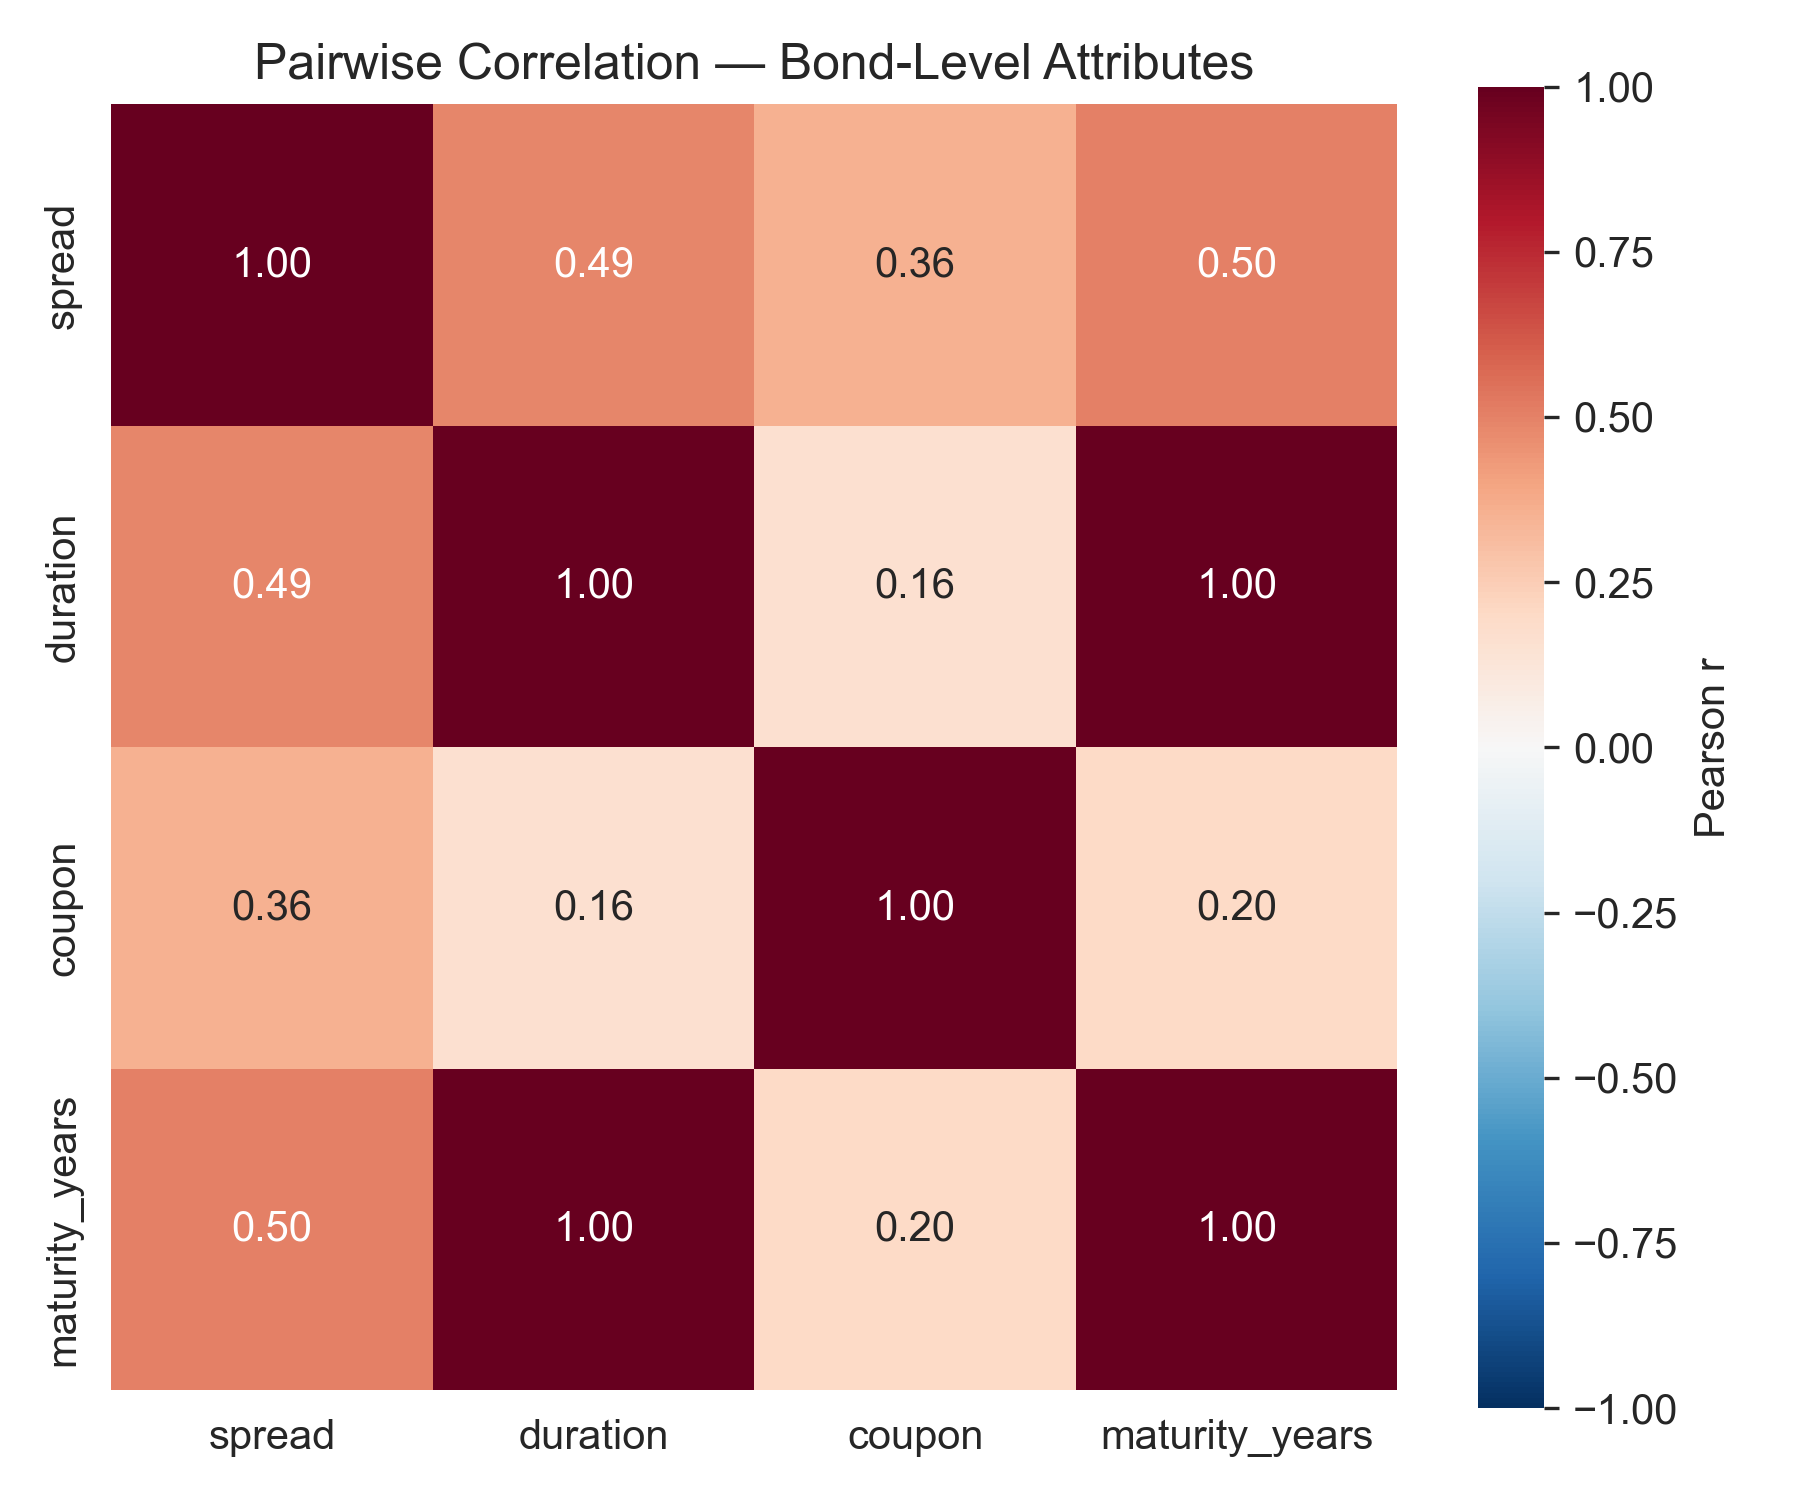
\includegraphics[width=0.7\linewidth]{outputs/figures/correlation_heatmap.png}
    \label{fig:corr_heatmap}
\end{figure}

\begin{table}[H]
\centering
\caption{Significance test results for spread drivers.}
\label{tab:significance_tests}
\begin{tabular}{lrr}
\toprule
Test & Statistic & p-value \\
\midrule
Pearson r (spread vs. duration) & 0.492000 & 0.000000 \\
Kruskal-Wallis (spread by rating) & 128.501000 & 0.000000 \\
Kruskal-Wallis (spread by sector) & 34.648000 & 0.000100 \\
\bottomrule
\end{tabular}

\end{table}

Spread and duration are significantly correlated (Pearson $r = 0.492$, $p < 0.001$), consistent with the OLS slope of 6.5 bps/year identified above. A Shapiro-Wilk test rejected normality of the spread distribution ($p < 0.001$), so a Kruskal-Wallis test was used in place of ANOVA: spread differs significantly across both rating cohorts ($H = 128.50$, $p < 0.001$) and BICS Level 1 sectors ($H = 34.65$, $p = 0.0001$). Tukey HSD post-hoc comparisons confirm that spread differences between coarse rating categories (e.g., AAA vs.\ BBB) are pairwise significant, while differences between adjacent notches within the same letter grade (e.g., A vs.\ A+) are generally not, consistent with the monotonic but noisy notch-level ordering observed in Figure 4.

% -------------------------------------------------------
% METHODOLOGY
% -------------------------------------------------------
\section{Methodology}

The methodology proceeds in three construction stages followed by an evaluation. First, raw Bloomberg price and static data are transformed into a clean panel of daily credit spreads. Second, a data pipeline aligns those spreads with bond attributes, cash flow schedules, modified durations, and regulatory capital factors to produce a complete set of optimizer inputs for any given valuation date. Third, a linear program selects an optimal bond portfolio against a fixed Funding Agreement-Backed Note (FABN) liability, jointly optimizing statutory investment income, capital efficiency, and transaction costs subject to duration, concentration, and cash flow constraints; an interest-rate swap overlay hedges the portfolio's exposure to the risk-free rate, so that the book can hold longer, higher-spread credit while remaining duration-matched to the note and compensated for credit risk rather than interest-rate movements. Finally, a walk-forward backtest re-solves the program on a rolling basis to evaluate the strategy against a passive benchmark. The subsections below describe each in turn.

\subsection{Feature Engineering}

The raw Bloomberg data provide only prices and static reference fields for each bond, which are insufficient for analyzing spread dynamics or for building a spread-based optimization engine. To resolve this, a daily spread over the risk-free curve is computed for every bond using the QuantLib fixed-income library. This requires calendarizing each bond's cash flow schedule, projecting coupon and principal payments on their exact settlement dates, and computing the annualized yield implied by the market price before differencing it against the risk-free curve at the matching tenor to obtain an option-adjusted spread (OAS). Accrued interest is incorporated into the dirty price used in the yield calculation, which stabilizes the resulting series by removing the mechanical sawtooth pattern introduced by coupon accrual between payment dates. The output is a clean panel of daily OAS observations per bond, suitable for both cross-sectional analysis and time-series modeling downstream.

\subsection{Modeling Frameworks}

\subsubsection{Pipeline}

The data pipeline assembles all optimizer inputs for a single valuation date from three source tables: static bond attributes, daily OAS spreads, and per-bond cash flow schedules. From these, it constructs the eligible bond universe, aligns spreads, and builds daily and quarterly cash flow matrices. Modified durations are computed from first principles from each bond's projected cash flows and a Treasury discount curve sourced from Federal Reserve Economic Data (FRED), rather than taken from vendor analytics, so that the duration used in the objective is internally consistent with the cash flows used in the constraints. Each bond is assigned a National Association of Insurance Commissioners (NAIC) C-1 asset-risk capital factor by credit rating, which quantifies the regulatory capital a holding consumes. The FABN liability schedule and its modified duration are derived directly from the contract terms. All outputs are collected into a single input object and passed to the optimizer after a validation step. This step checks dimensional consistency between the cash flow matrices and the bond universe, confirms spread coverage across the eligible set, fills any missing spreads with sector medians, and verifies that the assembled inputs are economically and accounting-consistent before optimization. A downstream feasibility check further confirms that the solved allocation satisfies every constraint. Figure 7 summarizes the end-to-end flow.

  % ── Figure 7: Pipeline Diagram ─────────────────────────
    \begin{figure}[H]
        \centering
        \caption{End-to-end data pipeline from raw Bloomberg inputs to the optimizer input set.}
        \label{fig:pipeline}
        \includegraphics[width=0.8\linewidth]{pipeline_diagram_white.png}
    \end{figure}

\subsubsection{Portfolio Optimization Model}

The portfolio is constructed under United States Statutory Accounting Principles (SAP), under which an insurer holds bonds at amortized cost and creates value through stable accrual earnings per unit of regulatory capital rather than through mark-to-market gains. The relevant profitability measure is therefore statutory net investment income (NII), coupon and accretion income net of the liability's funding cost, not price appreciation. This framing distinguishes the problem from a classical mean-variance formulation: the reward is income rather than expected return, risk enters through regulatory capital consumption and duration mismatch rather than return variance, and forced-sale liquidity is modeled explicitly. The problem is cast as a linear program (LP) with continuous holdings, which yields a globally optimal solution and exact dual prices and is solved with the Gurobi Optimizer.

The optimizer chooses two sets of nonnegative decision variables: the dollar amount $h_i$ allocated to each bond $i$ in the eligible universe ($i = 1, \dots, N$), and the notional $v_k$ of each candidate interest-rate swap at tenor $k$ ($k = 1, \dots, K$). The swaps constitute a pay-fixed overlay whose sole purpose is to hedge the book's interest-rate (duration) exposure; their construction and economic rationale are developed at the end of this subsection, but they are declared here because they enter the objective and constraints jointly with the bond holdings. Quarterly cash-flow and liquidity terms are indexed by $q = 1, \dots, Q$ over the horizon to the FABN's maturity, and the total budget backing the note is denoted $H$. The formulation additionally uses nonnegative auxiliary variables: the duration-gap slacks $d^{+}, d^{-}$, the per-quarter facility balance $B_q$ and residual shortfall $s_q$, and the turnover components $tc^{+}_i, tc^{-}_i$, each introduced together with the constraint that defines it below.

\paragraph{Objective Function.}

The program maximizes statutory NII net of capital and trading costs, with a facility reinvestment credit:
\begin{equation}
\begin{aligned}
\max_{h,\,v}\quad
& \underbrace{\sum_i (y_i - r_{\text{FABN}})\,h_i}_{\text{net investment income}}
\;-\; \underbrace{\lambda_{\text{cap}} \sum_i \theta_i\,h_i}_{\text{C-1 capital charge}}
\;-\; \underbrace{\lambda_{\text{cap}}\,\mu \sum_k v_k}_{\text{C-3 swap capital charge}} \\[4pt]
& \;-\; \underbrace{\sum_i \tau_i\,(tc^{+}_i + tc^{-}_i)}_{\text{turnover / bid-ask cost}}
\;+\; \underbrace{r_{\text{save}} \sum_{q<Q-1} \Delta t_q\,B_q}_{\text{facility reinvestment income}},
\end{aligned}
\end{equation}
where $y_i$ is bond $i$'s book yield, $r_{\text{FABN}}$ the FABN funding rate, $\theta_i$ the NAIC C-1 capital factor, $\tau_i$ the bid-ask half-spread, $DF_q$ the discount factor for quarter $q$, and $\Delta t_q$ the quarter length in years. The swap enters the objective only through a C-3 (interest-rate-risk) capital charge $\mu$ on its notional: struck at-the-money and modeled as a pure duration hedge, it carries no net income, consistent with its role of removing interest-rate risk rather than generating spread. Its fixed rate $c_k$ and the floating Secured Overnight Financing Rate (SOFR) proxy $r_{\text{float}}$ enter only through the swap's modified duration in the constraints below. The capital price $\lambda_{\text{cap}} = \text{cost\_of\_capital} \times \text{RBC\_bar}$ converts required capital into an income-equivalent charge, so the bond terms reward only spread earned in excess of both the funding cost and the cost of the capital a holding consumes.

\paragraph{Constraints.} 

The full budget is deployed,
\begin{equation}
\sum_i h_i = H,
\end{equation}
and the combined asset-plus-swap duration is held within a symmetric band around the liability's modified duration $D_{\text{FABN}}$, so the hedged book is interest-rate matched to the FABN. Because the pay-fixed swap carries negative duration, it offsets the rate sensitivity of longer bonds:
\begin{equation}
\sum_i D_i\,h_i - \sum_k D^{sw}_k\,v_k - D_{\text{FABN}}\,H = d^{+} - d^{-}, \qquad d^{+},\,d^{-} \le \varepsilon_D\,H.
\end{equation}
Here $D^{sw}_k < 0$ is the pay-fixed swap's modified duration at tenor $k$, set by its fixed rate $c_k$ and the floating rate $r_{\text{float}}$; struck at-the-money ($c_k = r_{\text{float}}$), the swap has zero value at inception and enters the model through this duration alone---no carry and no net cash flow. Turnover is linked to the current book $h^{\text{curr}}$ so that every change is costed,
\begin{equation}
h_i - h^{\text{curr}}_i = tc^{+}_i - tc^{-}_i,
\end{equation}
and a lending-facility recursion rolls surplus cash forward at $r_{\text{save}}$ each quarter, booking any gap as a shortfall:
\begin{equation}
B_q - s_q = (1 + r_{\text{save}}\,\Delta t_q)\,B_{q-1} + CF^{A}_q - CF^{L}_q,
\end{equation}
with $CF^{A}_q$ and $CF^{L}_q$ the asset and liability cash flows in quarter $q$ (the at-the-money swap contributes no net settlement). A liquidity safety cap bounds the present value (PV) of all shortfalls as a fraction of the liability's PV,
\begin{equation}
\sum_q DF_q\,s_q \le \varphi_{sf}\cdot \text{PV}(\text{liability}),
\end{equation}
an issuer-concentration cap limits any single issuer group $g$ to a share of the budget,
\begin{equation}
\sum_{i \in g} h_i \le \delta\,H,
\end{equation}
and the total swap notional is capped as a share of the budget:
\begin{equation}
\sum_k v_k \le \text{swap\_cap\_pct}\cdot H.
\end{equation}
Regulatory capital enters the model as a priced cost rather than a hard limit: the Risk-Based Capital a position consumes is charged in the objective through the C-1 and C-3 terms, consistent with the statutory view that capital is optimized against income rather than bounded outright. Bonds maturing after the FABN are admissible rather than excluded: the swap hedges the rate sensitivity of their sale price, so a bond that outlives the note and must be unwound before maturity is protected against adverse rate moves, leaving only the compensated credit exposure.

\paragraph{Parameters.} 

The base case uses a budget of $H = \$500$M, a funding rate $r_{\text{FABN}} = 3.205\%$, a liability duration $D_{\text{FABN}} = 3.24$ years, a duration band half-width $\varepsilon_D = 0.30$ years, an issuer cap $\delta = 5\%$, a capital price $\lambda_{\text{cap}} = 0.45$ (a $15\%$ cost of capital times a required-capital multiplier of $3$), and a PV-shortfall cap $\varphi_{sf} = 1\%$ that governs shortfalls as a hard limit rather than as an objective penalty. The reinvestment rate $r_{\text{save}}$ is set to $r_{\text{FABN}}$. The swap overlay uses a floating SOFR proxy $r_{\text{float}} = 4.35\%$ with fixed legs struck at-the-money ($c_k = r_{\text{float}}$), a C-3 capital charge $\mu = 0.002$ on notional, and a notional cap of $20\%$ of $H$. The bond-level inputs $y_i$, $\theta_i$, $\tau_i$, and the quarterly cash flows are produced by the pipeline. A complete parameter table is provided in Appendix~A.

\paragraph{Interest-Rate Swap Overlay.} 

The swap overlay is central to the strategy: it hedges the portfolio's exposure to the risk-free rate so that the FABN book is compensated for credit spread rather than for interest-rate movements. Each pay-fixed swap, struck at-the-money, pays the fixed rate $c_k$ against the floating SOFR proxy $r_{\text{float}}$ and is modeled as a pure duration hedge: it carries negative duration that offsets the rate sensitivity of the bond holdings while contributing no net carry to income. Because the swap strips out the rate exposure of the bonds, the optimizer can admit longer-duration, higher-spread credit that a duration-matched, bonds-only book could not hold, isolating the compensated credit exposure while the swap neutralizes the shared risk-free-rate risk. The residual risk the swap does not remove is the gap between book value and market value at the FABN maturity, when positions may have to be unwound to repay the note; this terminal gap, rather than exact cash-flow dedication, is the risk the formulation manages, through the duration match and the liquidity cap on shortfalls that together limit the loss realized if positions are unwound at maturity. A Conditional Value-at-Risk (CVaR) limit on this terminal book-to-market gap is the planned refinement of that control, bounding the tail loss at a forced unwind directly rather than through the duration and liquidity constraints alone. A bonds-only configuration, with the swap notional held at zero, provides the natural comparison point in the backtest.

\subsubsection{Walk-Forward Backtesting}

To evaluate the strategy over time rather than at a single date, the program is embedded in a walk-forward backtest that re-solves it on a rolling basis, re-optimizing the book at a fixed cadence and holding it fixed between re-optimizations. On each date the model chooses between buy $b_i \ge 0$ and sell $0 \le s_i \le h^{\text{prev}}_i$ relative to the previous book, so that $h_i = h^{\text{prev}}_i + b_i - s_i$. Retained notional keeps its locked-in book yield while new purchases enter at the prevailing market yield, reflecting the amortized-cost treatment under SAP. Realized gains or losses from rate-driven sales are not booked at the trade date but placed in an Interest Maintenance Reserve (IMR) and amortized into income over the sold bond's remaining life, consistent with statutory practice; the reserve is an accounting consequence and does not alter the trade the optimizer selects. Income and capital are valued over the remaining horizon to maturity, so that a one-time trade cost is judged against the income a holding would actually earn; this discourages both excessive churning and complete freezing of the book. A trading-cost hurdle multiplier scales the bid-ask charge to widen a no-trade band and suppress marginal, low-value trades.

Two mechanisms keep the rolling program feasible and realistic. The duration band is softened: deviations beyond $\varepsilon_D$ are permitted but penalized, so the LP remains feasible in early periods when the liability is long relative to the available universe, while behaving identically to the hard band whenever the band is reachable. Residual shortfalls that the facility cannot cover are financed at a borrowing rate and penalized, distinguishing the cost of a genuine cash gap from ordinary reinvestment. The reinvestment policy is made explicit rather than implicit: principal returned by maturing bonds accumulates in the lending facility and is redeployed into the bond universe at the next re-optimization under a stated reinvestment rate, so that the sequential nature of the problem is represented directly rather than assumed away. The strategy is benchmarked against a passive baseline that deploys the budget once and holds it to maturity, so that the incremental value of active, constraint-aware re-optimization can be isolated. Performance is assessed along four dimensions: net economic value relative to the baseline, the statistical significance of that advantage, portfolio turnover, and constraint utilization inferred from the LP dual prices, which are defined here and quantified in the Findings section.




% -------------------------------------------------------
% CONCLUSION
% -------------------------------------------------------

\section{Results}

\subsection{Optimization Results}

The walk-forward backtest establishes the two anchors against which every other number is read. A passive, buy-and-hold static book, the industry-standard baseline, produces \$27.76M of cumulative net statutory income (net interest income plus trading gains) over the two-year window. A realistic, tuned dynamic strategy that re-optimizes on a monthly cadence with a transaction-cost hurdle lifts this to approximately \$31M, an improvement of roughly \$3.2M (about +11–12\%) earned purely through disciplined rebalancing, with no relaxation of the duration, capital, or concentration constraints. This confirms the project's core hypothesis in the affirmative but modest direction: adaptive reoptimization does beat the static baseline, and it does so without violating any regulatory or ALM limit.

% ── Figure 8 ──
\begin{figure}[H]
    \centering
    \caption{Cumulative NII, IMR balance, and realized vs. recognized gains under the dynamic path.}
    \label{fig:nii-imr-realized}
    \includegraphics[width=\linewidth]{1. Cumulative Net Statutory Income — Static vs Dynamic (base & tuned).png}
\end{figure}

The realized \$3.2M raises the natural business question a prospective client asks: is that the ceiling, or is there substantially more value being left on the table? To answer it we compute a perfect-foresight upper bound: the maximum cumulative net statutory income and a re-optimizing trader could ever book if the entire future price path were known in advance. This is deliberately not a strategy (foresight is unattainable); it is a ceiling, and its business value is the gap to the realistic dynamic result. Formulated as a time-expanded "trade-arc" linear program that conserves book value (so realized gains can never inflate redeployable principal), the foresight model produces, on a monthly rebalance grid, a prize of \$41.99M windowed (\$62.26M if the full, ultimately-recognized trading gains release is credited). Two internal checks validate the construction: the foresight static floor of \$27.76M and the model asserts the required ordering (prize ≥ foresight-static ≥ realized) as an upper bound. The headline reads as follows. The value attributable purely to timing (foresight dynamic minus foresight static) is \$14.23M (+48.6\%), and the head-room between the realistic dynamic strategy (~\$31M) and the ceiling is roughly \$13M (+35\%) on a monthly grid, widening to \$11–23M (+35–75\%) as the grid refines toward weekly. In short: there is real, tradeable upside beyond what the current rules-based strategy captures, so the problem is worth continuing to build.

The most important, and least obvious result is the decomposition of the prize into its sources. Carry income is essentially identical between the static and dynamic solutions (about \$32.7M static versus \$32.9M dynamic): the static book already owns virtually all of the available carry. The entire dynamic edge comes instead from realized, rate-driven gains harvested through trading and recognized via the Interest Maintenance Reserve (IMR): \+\$16.27M on a monthly grid, bought with roughly \$4.8M of incremental transaction cost against a small \$2.4M capital charge. The prize is therefore a rate-rotation-timing story, not a bond-selection story. Because IMR amortizes a realized gain over the sold bond's remaining life rather than booking it at once, a two-year window understates the effect, hence the gap between the \$42M windowed and \$62M fully-recognized figures. A subtle but consequential corollary is that IMR and NII are structurally in tension: selling a bond to harvest an IMR gain simultaneously terminates its carry, so dynamic trading does not simply add IMR on top of carry, it partially substitutes for it (the two are anti-correlated at r = −0.411 in monthly data).

% ── Figure 9 ──
\begin{figure}[H]
    \centering
    \caption{Static vs. dynamic component decomposition and net prize by rebalance granularity.}
    \label{fig:static-dynamic-decomp}
    \includegraphics[width=\linewidth]{3. Static vs Dynamic Decomposition (Monthly Grid).png}
\end{figure}

The foresight solution is not a churning machine; it trades with high precision. It opens 211 active arcs totaling about \$4.7B of notional on a \$500M book (roughly 9.5× turnover over two years), of which 95.3\% are profitable. The optimizer almost never makes a losing trade. The median arc earns about 67.5 bps per dollar, and the mean hold is 76 days, indicating multi-month strategic positions rather than high-frequency flips. Hold duration is in fact the single strongest predictor of arc profit (r = 0.789): the primary lever is patient, medium-term positioning, not rapid round-trips. Trading is volatility-triggered rather than volatility-proportional, the linear correlation between weekly trade count and yield volatility is near zero (r = 0.044), yet 9 of the 10 heaviest trading weeks fall in the highest-volatility periods. The book sits quiet through calm regimes and fires concentrated bursts only when volatility is extreme.

% ── Figure 10 ──
\begin{figure}[H]
    \centering
    \caption{Size of the prize vs. rebalance grid density.}
    \label{fig:prize-granularity}
    \includegraphics[width=0.8\linewidth]{2. Size of the prize vs rebalance granularity.png}
\end{figure}

Because trade opportunities scale with how finely time is sampled, we sweep the rebalance grid from quarterly to weekly. The prize rises monotonically quarterly \$36.2M, monthly \$42.0M, biweekly \$47.1M, weekly \$54.0M windowed, but with strongly diminishing returns: a fitted power law gives an exponent of only α = 0.164 (R² = 0.994), meaning that doubling the rebalancing frequency adds only about 12\% more prize. Every refinement step remains net-positive after costs; on average each \$1 of transaction cost spent earns \$2.77 of IMR (R² = 0.986). Monthly is the most cost-efficient grid (IMR-to-cost ratio of 3.39×) and is the conservative number we quote as the defensible prize. A deliberately extreme "daily × full universe" run illustrates where the assumptions break: at a 10-day maximum hold the model trades about \$52B on the \$500M book (~100× turnover) to harvest a headline \$96M — but our cost model charges only half the bid-ask spread with zero market impact, and no insurer can trade 100× its assets. That figure is an artifact of the no-impact assumption, not a business target, and it is precisely why a market-impact cost is the natural next modeling step. Finally, turning the lending-facility and PV-shortfall constraints on leaves the prize unchanged with zero borrowing cost, confirming that liquidity is not the binding constraint the duration band and concentration limits are.
A model-free ranking of each bond's IMR opportunity (spread range × duration, per unit of C-1 capital) shows that high-quality, long-duration bonds (AAA/AA+) dominate IMR generated per dollar of regulatory capital by a wide margin, because their C-1 charge is small relative to their spread volatility. The implication for strategy is counterintuitive: if the duration band or issuer cap is loosened, the capital-efficient path to IMR is to reach for high-quality duration, not for BBB spread.


% ── Figure 11 ──
\begin{figure}[H]
    \centering
    \caption{Cumulative net statutory income: static vs. dynamic (base and tuned).}
    \label{fig:cumulative-net-static-dynamic}
    \includegraphics[width=\linewidth]{4. Realized vs recognized — tuned (IMR re-times the gain).png}
\end{figure}

\subsection{Product}
\subsubsection{\textit{Dashboard }}

The dashboard is a single-page React and TypeScript application backed by a Python FastAPI service, giving the portfolio manager one working surface for the FABN under management rather than a static report. Its central panel presents portfolio KPIs organized into three views: the FABN's spread and crediting rate against market benchmarks, a lender's-eye return-on-equity view (statutory NII, the SAP objective, C1 usage, and required regulatory capital), and portfolio-level metrics including duration, historical-simulation CVaR, and capital efficiency. Adjoining tabs surface the optimizer's other outputs: a Suggested Trades view listing the buy and sell candidates ranked by their marginal contribution to the SAP objective, a Risk view showing the CVaR distribution alongside a percentile-based volatility trading signal, a Strategy Tracking view exposing shadow prices on the duration, budget, and issuer-concentration constraints together with per-bond reservation prices, and a Derivative Usage view for the swap overlay. A sidebar lets the user adjust the optimizer's hyperparameters, cost of capital, the savings-rate scalar, the duration-gap tolerance, the maximum single-bond weight, and the minimum bond count, and reissue the solve with those values.

Data reaches the frontend through a set of versioned FastAPI routers rather than a single aggregate call. Bond metadata and spreads are read from BigQuery, market rates and news pass through Alpaca with VADER-based sentiment scoring, and the optimizer itself is exposed through a single endpoint that runs the Gurobi-based linear program on a worker thread so the solve does not block the event loop. Because each solve first rebuilds the bond universe and cash-flow schedule for the requested date, that intermediate pipeline output is cached in memory per date, so repeated solves for a date already visited in the session, for instance after changing a hyperparameter, skip the BigQuery round-trip and re-solve directly. Constraint status shown in the Risk tab, covering the budget, duration gap, present-value shortfall, and held-to-maturity exclusions, is computed by the optimizer itself and passed through unchanged, so the dashboard never re-derives or approximates a figure the solver already produced. Trades a user chooses to act on are recorded through a dedicated endpoint that overrides the affected CUSIPs' current holdings for the remainder of the session; this blotter is held in server memory only and is reset explicitly, rather than persisted to a database, since its purpose is to let a manager simulate acting on the optimizer's suggestions rather than to book real trades.

Several parts of the dashboard are explicitly scaffolded rather than fully live. The FABN selector lists the single note the pipeline actually models alongside additional entries marked as forthcoming and disabled, reflecting that the underlying data pipeline and optimizer presently cover one funding agreement. Market rates and news fall back to a fixed, clearly labeled stub feed only when the external market data provider is unreachable, and portfolio KPIs that require an actual optimizer solve fall back to a labeled stub state before any date has been optimized. This distinction between a live, optimizer-derived figure and a placeholder value is carried into the interface itself, where every KPI is tagged as either optimizer-backed or stubbed so that a user is never shown a number that only appears to come from a completed solve.

\subsubsection{\textit{Agent }}

The FABN agent acts as a conversational layer on top of the portfolio optimizer, translating natural-language requests into structured actions and turning structured results back into plain-English answers without ever letting the language model touch the financial computation. A user message first passes through a routing step, where an open source large language model (Qwen2.5) classifies the request into one of three intents: \textit{run} (configure and execute an optimization), \textit{select} (retrieve results from the most recent run), or \textit{explain} (answer a conceptual question about how the model works). This classification is returned as a small structured JSON object rather than free text, so every downstream step operates on validated, typed data instead of raw language.

Each intent is handled deterministically once identified. A \textit{run} request is checked against business rules (valid dates, positive budgets, sensible risk parameters) before being mapped onto the optimizer's actual inputs; the solve itself is executed by the underlying linear program, with the language model playing no role in the math. A \textit{select} request pulls from a fixed set of pre-defined queries, including summary metrics, position changes and recommended trades, with no model-generated logic in between. This separation allows the optimizer's outputs to be reproducible and auditable, so the language model is only an interface to, not a participant in, the calculation. The \textit{explain} intent lets users ask open-ended "why" questions; for instance: “If we intentionally reduce our swap notional so that our duration hedge is slightly under-matched relative to target, how does that affect our P\&L, and why? Walk me through the mechanism and give a concrete example" and, “I am considering rebalancing the duration hedge weekly instead of monthly. What are the trade-offs of moving to a weekly cadence, and what is your recommendation and why?”

Rather than relying on the model's general knowledge, the agent grounds each answer in two reference documents describing the portfolio's duration and hedging logic and its optimization formulation, along with the numeric results of the user's own most recent run, if one exists. The documents explicitly distinguish between mechanisms that are currently implemented and those that are only planned, and the model is instructed to preserve that distinction rather than blur it, so an explanation cannot imply that a feature is live when it is not. Together, these three pathways let the agent serve as an accessible interface for a regulated, math-heavy optimization system. It is fast enough for exploratory questions, but structured so that financially consequential information runs through the same deterministic, auditable pipeline every time.


To be filled out when we get some results.

\section{Discussion}

Several practical considerations qualify these results. The realized \$3.2 million improvement over the static baseline required no relaxation of duration, capital, or concentration constraints, so the gain is available within an insurer's existing risk appetite. This value comes with a direct rebalancing-frequency tradeoff: the prize rose from \$36.2 million quarterly to \$54.0 million weekly, but with strongly diminishing returns, so the monthly cadence was adopted as the most cost-efficient and defensible figure rather than the theoretical maximum. The decomposition further showed that carry income was nearly identical between the static and dynamic books, meaning the entire dynamic edge came from realized trading gains through the IMR, and that these two income sources are structurally in tension rather than additive. The framework also implied that, if constraints were loosened, the capital-efficient response is to extend into high-quality duration rather than lower-rated spread, since AAA/AA+ bonds generated more IMR opportunity per unit of regulatory capital.

The analysis carries several limitations. The perfect-foresight ceiling assumes complete knowledge of the future price path and is intended only to bound attainable value, not to represent a usable strategy; an extreme daily-rebalancing configuration illustrated this by requiring roughly 100 times turnover to reach its headline prize, a level no insurer could execute, and pointed to market-impact cost as a necessary next modeling step. The results are further bounded by the project's scope: a single FABN structure under U.S. regulation over a two-year window, a swap overlay without a terminal book-to-market risk control beyond duration matching and the liquidity cap, and a news-sentiment signal that returned no statistically significant relationship with issuer spreads and so could not yet be validated as a reoptimization trigger.

\section{Conclusion}

\subsection{Use Case for Client}

A first application to Athene Global Funding's Series 2022-6 FABN (\$500M outstanding, 3.205\% due March 2027) and the 303-bond investment-grade universe described in Section 3, the Gurobi-based optimizer produced a 21-bond allocation with a portfolio weighted-average duration of 2.1896 years — within the prescribed band around $D^{FABN}$ — and an RBC ratio of 1.50x, satisfying the minimum capital adequacy requirement. The resulting net economic value was \$14,554,820.29, demonstrating that meaningful spread capture is achievable within the regulatory and ALM constraints that characterize institutional FABN portfolio management. Sensitivity analyses across the RBC ratio, duration tolerance band, and issuer concentration cap further illustrated the trade-offs embedded in the constraint structure, providing the client with an initial basis for calibrating these parameters to their specific risk appetite.

In parallel, a proof-of-concept dashboard and agentic layer were prototyped as the intended end-user interface. The dashboard integrated a React/TypeScript frontend with a Python FastAPI backend and Google BigQuery, surfacing portfolio KPIs, optimizer-generated trade recommendations, and real-time market news alongside risk constraint status. A proposed agentic architecture — grounding a tool-using language model over the optimization pipeline via LangGraph and FastAPI — was designed to translate optimizer outputs into plain language and allow end users to explore scenarios interactively, without direct access to the solver. Full AI integration and walk-forward backtesting represent the primary milestones toward a production-ready deployment. Beyond the FABN use case, the RBC-constrained optimization framework is directly extensible to other insurance-backed structured notes and analogous institutional settings — including pension fund ALM and bank treasury operations — where portfolio management requires joint optimization of spread generation, liability matching, and regulatory capital efficiency.

\subsection{Next Steps}

Walk-forward backtesting over the two-year Bloomberg dataset remains the primary outstanding validation milestone. This entails running the optimizer on a daily cadence, ingesting daily bond prices alongside existing spreads and cash flows, and comparing cumulative NEV, RBC utilization, and duration compliance between the dynamic strategy and a static buy-and-hold baseline to assess whether the adaptive approach generates measurable outperformance. In parallel, the framework would be extended to optimize across multiple FABN tranches simultaneously, which smooths terminal-quarter cash flow concentration risk and allows surplus from one FABN to offset shortfalls in another without relying on the lending facility. On the risk management dimension, convexity matching would be promoted to a base-model constraint, complemented by key-rate duration alignment at the 1Y, 2Y, 3Y, and 5Y tenors and derivative overlays — including interest rate swaps, Treasury futures, and CDS positions — to decouple asset selection from duration and convexity management.

The client also identified a migration toward Statutory Accounting Principles as a key objective function enhancement. This would replace the current spread-based NEV maximization with a book-yield-driven net investment income formulation, decomposing returns into coupon, amortization, and realized gain components and incorporating expected credit loss as an explicit cost term. Asset Valuation Reserve and Interest Maintenance Reserve dynamics represent a further extension once the core SAP-faithful objective is validated. Additionally, the fixed income market signals introduced in the Analysis Goals and implemented as inactive override blocks in Section 4 — yield curve PCA, mean reversion across bond pairs, and capital structure relative value — remain to be activated, parameterized, and validated through the backtesting framework. News-based sentiment scoring, evaluated using FinBERT over Alpaca-sourced headlines, returned no statistically significant correlation with issuer-level spreads in initial testing ($Pearson-r = -0.03$, $p-value = 0.80$); domain-adapted filtering — including removal of non-financial articles and evaluation of fixed-income-specific models — remains a prerequisite before sentiment signals can serve as supplementary reoptimization triggers. Successful completion of backtesting will represent the primary empirical basis for evaluating whether the dynamic reoptimization approach generates measurable outperformance over the static buy-and-hold baseline established as the project's central performance objective.

An additional next step which is already in development is a light-weight agentic orchestration agent. The agent would serve as a natural language interface on top of the existing pipeline optimization pipeline, allowing end users to run or inspect the optimization, interpret results, and connect portfolio decisions to trades and market news without reading raw logs. A core guiding principle in the development of this agentic component is clearly defining and constraining agent behavior to a predefined set of scenario or question types, executing user-defined tasks without altering the existing Gurobi solver logic or portfolio math.

A potential agentic architecture could include LangGraph/LangChain or LlamaIndex as an agent orchestration framework, and LLM (Anthropic/OpenAI) as a reasoning engine that decides on tool usage, FastAPI as a backend server, and Pydantic for structure, validation, and schema definition. With this workflow or a similar one, the agent will reason within a constrained environment to enrich the end-user experience while the underlying structure minimizes risk.

% -------------------------------------------------------
% REFERENCES
% -------------------------------------------------------
\newpage
\section{References}

\renewcommand{\section}[2]{}
\printbibliography

% -------------------------------------------------------
% APPENDICES  (do NOT start each additional appendix on a new page)
% -------------------------------------------------------
% -------------------------------------------------------
% APPENDIX A — OPTIMIZER PARAMETERS
% -------------------------------------------------------
\newpage
\section*{Appendix A. Optimizer Parameters}

% Force appendix-style table numbering (Table A1, A2, ...) per the guide.
\setcounter{table}{0}
\renewcommand{\thetable}{A\arabic{table}}

Table~\ref{tab:params} lists the base-case parameters of the FABN portfolio optimizer, grouped into the core model, the swap overlay, and the walk-forward backtest.

\begin{table}[H]
\centering
\caption{Base-case parameters of the FABN portfolio optimizer.}
\label{tab:params}
\begin{tabular}{@{}lll@{}}
\toprule
\textbf{Symbol} & \textbf{Value} & \textbf{Description} \\
\midrule
\multicolumn{3}{@{}l}{\textit{Core model}} \\
$H$ & \$500\text{M} & Capital budget backing the FABN \\
$r_{\text{FABN}}$ & 3.205\% & FABN funding (liability) rate \\
$D_{\text{FABN}}$ & 3.24 yr & FABN modified duration \\
$\varepsilon_D$ & 0.30 yr & Duration-band half-width \\
$\delta$ & 5\% & Issuer-concentration cap (share of $H$) \\
$\lambda_{\text{cap}}$ & 0.45 & Capital price ($=$ cost of capital $\times$ RBC\_bar) \\
cost\_of\_capital & 15\% & Insurer cost of capital \\
RBC\_bar & 3 & Required-capital multiplier on C-1 \\
$\varphi_{sf}$ & 1\% & PV-shortfall cap (fraction of liability PV) \\
$r_{\text{save}}$ & $= r_{\text{FABN}}$ & Facility reinvestment rate \\
\midrule
\multicolumn{3}{@{}l}{\textit{Swap overlay (pay-fixed, receive-floating)}} \\
tenors $k$ & 1, 2, 3 yr & Pay-fixed swap tenors \\
$c_k$ & $= r_{\text{float}}$ & Fixed rate struck at-the-money (zero carry) \\
$r_{\text{float}}$ & 4.35\% & Floating leg (SOFR proxy) \\
$\mu$ & 0.002 & C-3 capital charge on swap notional \\
swap\_cap\_pct & 20\% & Cap on total notional (share of $H$) \\
\midrule
\multicolumn{3}{@{}l}{\textit{Walk-forward backtest}} \\
reopt\_every & 5 days & Re-optimization cadence (weekly) \\
$\kappa$ & $\ge 1$ & Trading-cost hurdle (no-trade band) \\
dur\_pen & 1.0 & Soft duration-band penalty \\
$r_{\text{borrow}}$ & 5\% & Borrowing rate on residual shortfalls \\
\bottomrule
\end{tabular}
\end{table}

%\section{Appendix B: [Title of Appendix B]}

%[Supporting material for Appendix B.]

\end{document}